% !Mode:: "TeX:UTF-8" (encoding info for WinEdt)
\section{Lien avec une base de données externe}
Lors du premier démarrage Elexis va créer de façon standardisé une base de données HSQL locale index{Server!Hsql}. On peut par contre sans problèmes aussi connecter à une autre base de données localement ou sur un autre ordinateur et ceci même à travers Internet (même si pour des raison de sécurité nous ne pouvons le conseiller que sous certaines condtions) 
Veuillez créer d'abdord une base de données vide sur votre ordinateur qui servira comme serveur. Supposons que le serveur ait l'adresse 192.168.0.2. Pour MySQL l'installation est décrit ci-joint en détail. Pour d'autres bases de données veuillez procéder en analogie.

\subsection{Créer base de données}
\index{Server!Connexion avec une base de données Mysql}
Veuillez vous connecter au serveur et introduire ensuite le suivant :

\begin{quote}
mysql -u root
\end{quote}

ceci ouvre le console mysql (... si vous avez installé correctement mysql).
Veuillez y introduire:

\begin{quote}
create database elexistest;

grant all on elexis.* to testuser@'\%' identified by 'testelexis';
\end{quote}

(Vous êtes naturellement libre d'utiliser un autre nom de base de données et un autre nom d'utilisateur de même que un autre mot de passe.)

Veillez démarrer ensuite Elexis et choisissez dans le menu 'fichier' -> connexion.

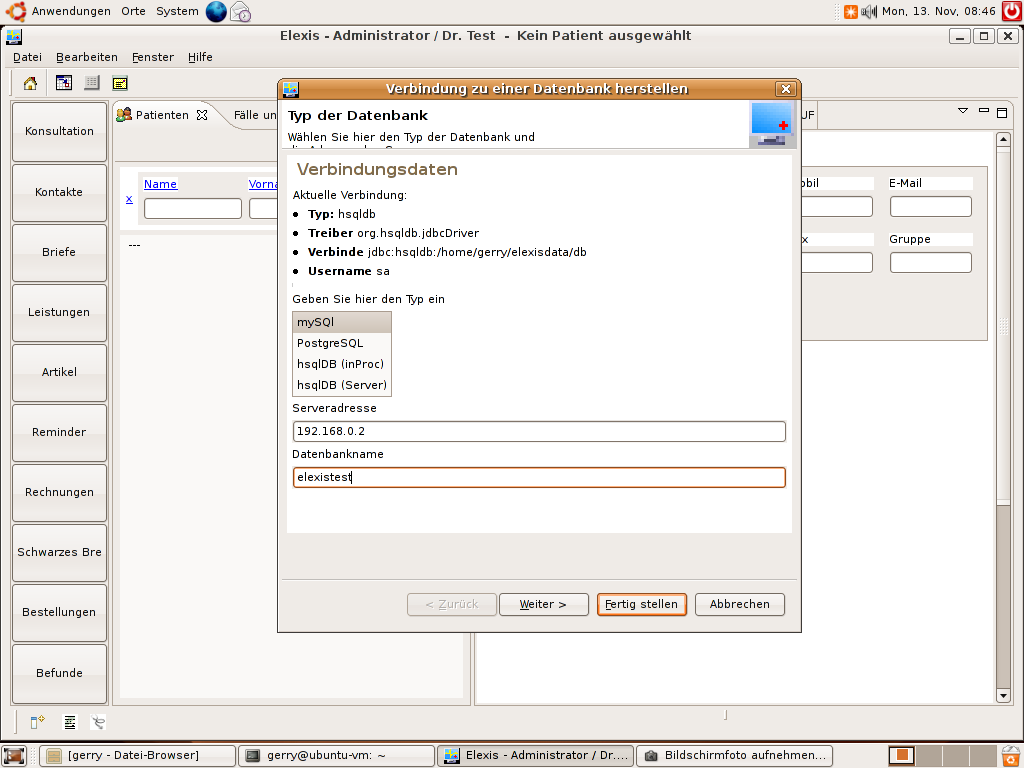
\includegraphics[width=4in]{images/verbindung11.png}
% verbindung11.png: 1024x768 pixel, 72dpi, 36.12x27.09 cm, bb=0 0 1024 768



Veuillez introduire le type de base de données(ici mysql),l'adresse du serveur (ici 192.168.0.2) ou son adresse Internet (par ex.  testserver.elexis.ch) de même que le nom de la base de données (ici  elexistest) et cliquez sur \textit{continuer}.

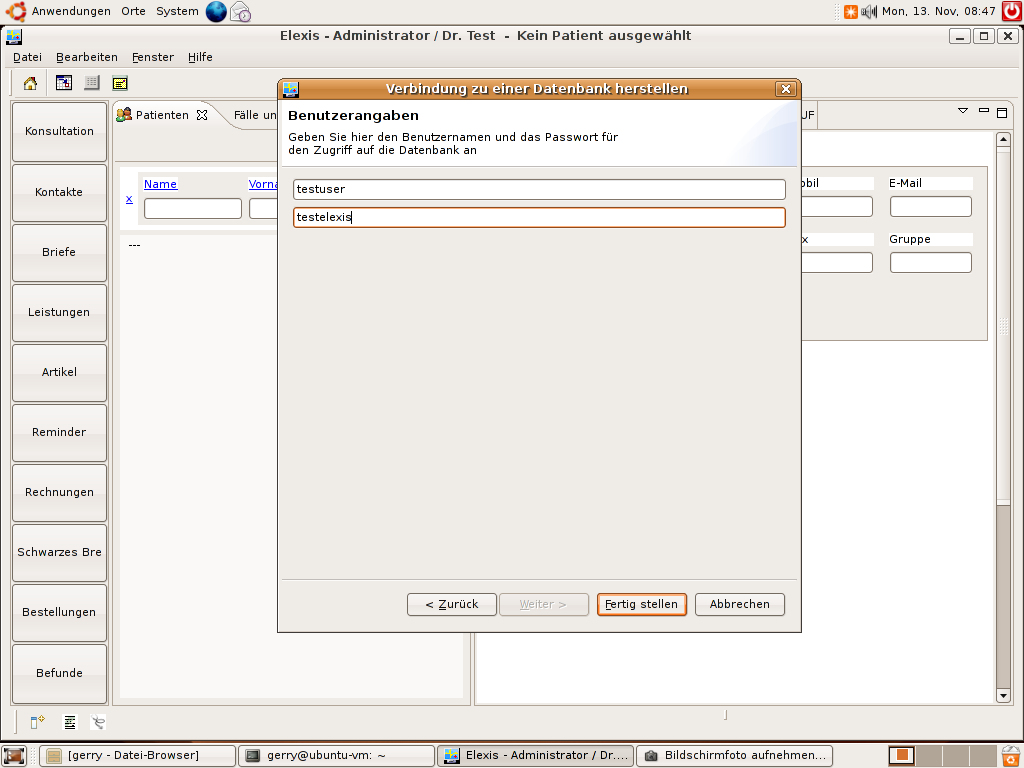
\includegraphics[width=4in]{images/verbindung12.png}
% verbindung12.png: 1024x768 pixel, 72dpi, 36.12x27.09 cm, bb=0 0 1024 768
Veuillez introduire dans la ligne supérieure le nom de l'utilisateur de la base de données (ici testuser) et dans la ligne inférieure le nom de passe correspondant (ici testelexis) et cliquez sur \textit{terminer}.

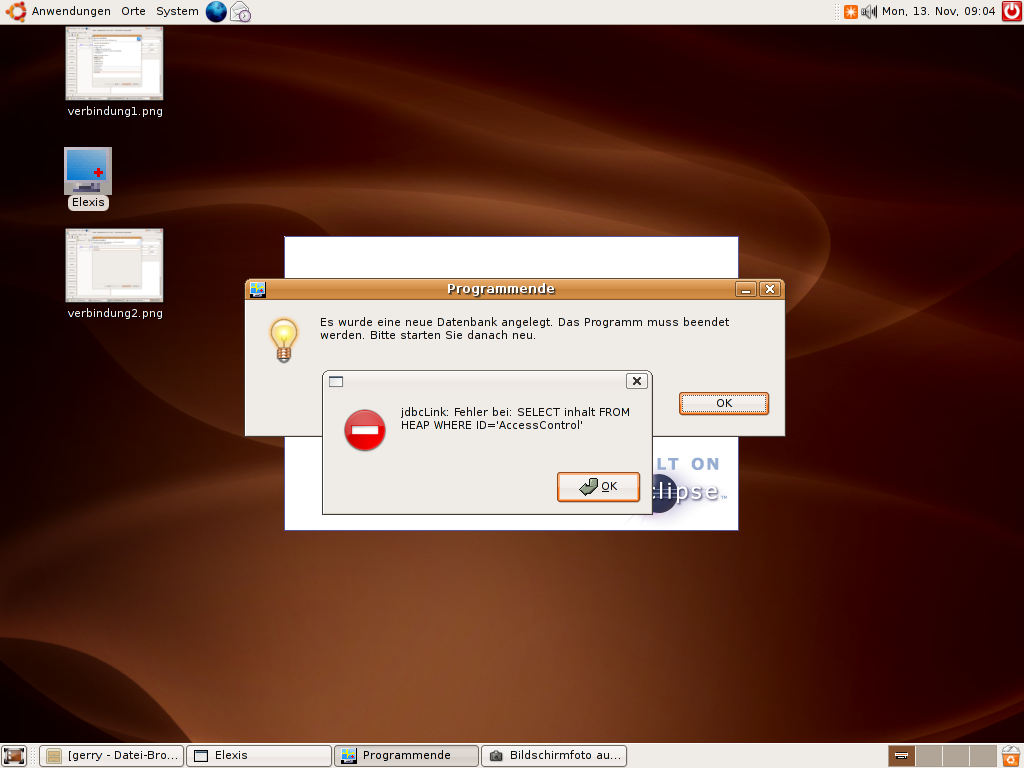
\includegraphics[width=4in]{images/verbindung13.png}
% verbindung13.png: 1024x768 pixel, 72dpi, 36.12x27.09 cm, bb=0 0 1024 768

 Il y aura quelques messaged d'erreur que vous pouvez fermer et ensuite il faudra redémarrer le logiciel.

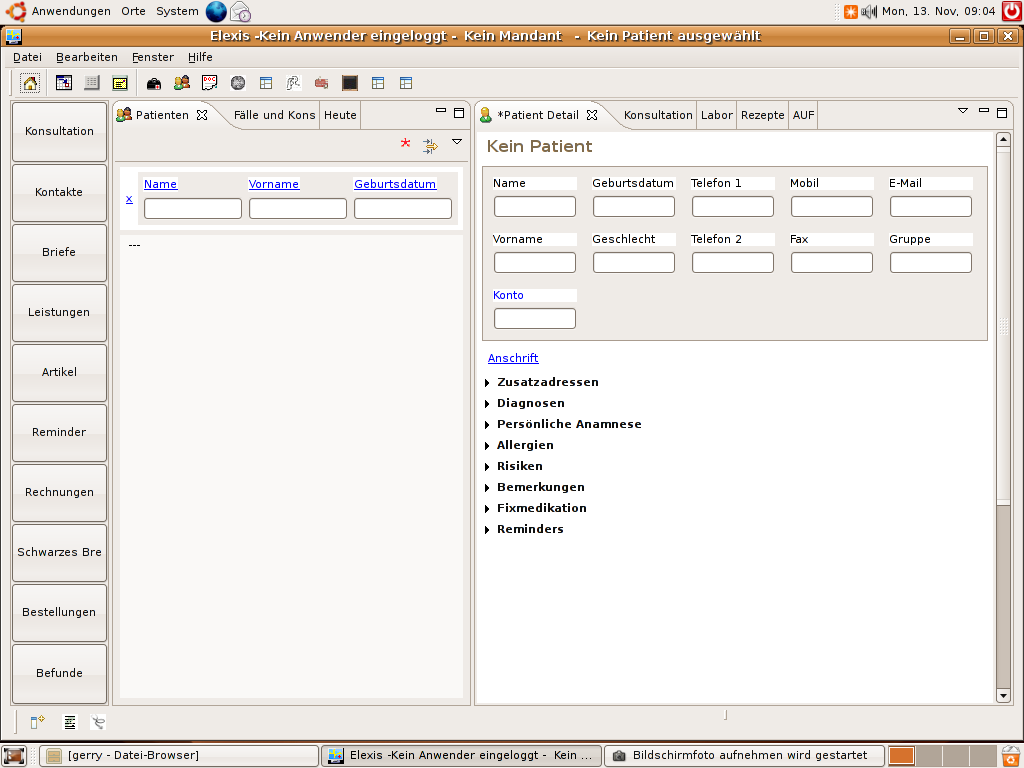
\includegraphics[width=4in]{images/verbindung14.png}
% verbindung14.png: 1024x768 pixel, 72dpi, 36.12x27.09 cm, bb=0 0 1024 768

Maintenant vous pouvez vous annoncer avec le nom \textit{Administrator} et le mot de passe \textit{admin} dans votre système Elexis que vous venez d'installer.

